\documentclass[10,]{article}
\usepackage{lmodern}
\usepackage{amssymb,amsmath}
\usepackage{ifxetex,ifluatex}
\usepackage{fixltx2e} % provides \textsubscript
\ifnum 0\ifxetex 1\fi\ifluatex 1\fi=0 % if pdftex
  \usepackage[T1]{fontenc}
  \usepackage[utf8]{inputenc}
\else % if luatex or xelatex
  \ifxetex
    \usepackage{mathspec}
  \else
    \usepackage{fontspec}
  \fi
  \defaultfontfeatures{Mapping=tex-text,Scale=MatchLowercase}
  \newcommand{\euro}{€}
\fi
% use upquote if available, for straight quotes in verbatim environments
\IfFileExists{upquote.sty}{\usepackage{upquote}}{}
% use microtype if available
\IfFileExists{microtype.sty}{%
\usepackage{microtype}
\UseMicrotypeSet[protrusion]{basicmath} % disable protrusion for tt fonts
}{}
\makeatletter
\@ifpackageloaded{hyperref}{}{%
\ifxetex
  \usepackage[setpagesize=false, % page size defined by xetex
              unicode=false, % unicode breaks when used with xetex
              xetex]{hyperref}
\else
  \usepackage[unicode=true]{hyperref}
\fi
}
\@ifpackageloaded{color}{
    \PassOptionsToPackage{usenames,dvipsnames}{color}
}{%
    \usepackage[usenames,dvipsnames]{color}
}
\makeatother
\hypersetup{breaklinks=true,
            bookmarks=true,
            pdfauthor={Patrik Nyman},
            pdftitle={Numeriska metoder, laboration 2},
            colorlinks=true,
            citecolor=blue,
            urlcolor=blue,
            linkcolor=magenta,
            pdfborder={0 0 0}
            }
\urlstyle{same}  % don't use monospace font for urls
\usepackage{color}
\usepackage{fancyvrb}
\newcommand{\VerbBar}{|}
\newcommand{\VERB}{\Verb[commandchars=\\\{\}]}
\DefineVerbatimEnvironment{Highlighting}{Verbatim}{commandchars=\\\{\}}
% Add ',fontsize=\small' for more characters per line
\newenvironment{Shaded}{}{}
\newcommand{\KeywordTok}[1]{\textcolor[rgb]{0.00,0.44,0.13}{\textbf{{#1}}}}
\newcommand{\DataTypeTok}[1]{\textcolor[rgb]{0.56,0.13,0.00}{{#1}}}
\newcommand{\DecValTok}[1]{\textcolor[rgb]{0.25,0.63,0.44}{{#1}}}
\newcommand{\BaseNTok}[1]{\textcolor[rgb]{0.25,0.63,0.44}{{#1}}}
\newcommand{\FloatTok}[1]{\textcolor[rgb]{0.25,0.63,0.44}{{#1}}}
\newcommand{\ConstantTok}[1]{\textcolor[rgb]{0.53,0.00,0.00}{{#1}}}
\newcommand{\CharTok}[1]{\textcolor[rgb]{0.25,0.44,0.63}{{#1}}}
\newcommand{\SpecialCharTok}[1]{\textcolor[rgb]{0.25,0.44,0.63}{{#1}}}
\newcommand{\StringTok}[1]{\textcolor[rgb]{0.25,0.44,0.63}{{#1}}}
\newcommand{\VerbatimStringTok}[1]{\textcolor[rgb]{0.25,0.44,0.63}{{#1}}}
\newcommand{\SpecialStringTok}[1]{\textcolor[rgb]{0.73,0.40,0.53}{{#1}}}
\newcommand{\ImportTok}[1]{{#1}}
\newcommand{\CommentTok}[1]{\textcolor[rgb]{0.38,0.63,0.69}{\textit{{#1}}}}
\newcommand{\DocumentationTok}[1]{\textcolor[rgb]{0.73,0.13,0.13}{\textit{{#1}}}}
\newcommand{\AnnotationTok}[1]{\textcolor[rgb]{0.38,0.63,0.69}{\textbf{\textit{{#1}}}}}
\newcommand{\CommentVarTok}[1]{\textcolor[rgb]{0.38,0.63,0.69}{\textbf{\textit{{#1}}}}}
\newcommand{\OtherTok}[1]{\textcolor[rgb]{0.00,0.44,0.13}{{#1}}}
\newcommand{\FunctionTok}[1]{\textcolor[rgb]{0.02,0.16,0.49}{{#1}}}
\newcommand{\VariableTok}[1]{\textcolor[rgb]{0.10,0.09,0.49}{{#1}}}
\newcommand{\ControlFlowTok}[1]{\textcolor[rgb]{0.00,0.44,0.13}{\textbf{{#1}}}}
\newcommand{\OperatorTok}[1]{\textcolor[rgb]{0.40,0.40,0.40}{{#1}}}
\newcommand{\BuiltInTok}[1]{{#1}}
\newcommand{\ExtensionTok}[1]{{#1}}
\newcommand{\PreprocessorTok}[1]{\textcolor[rgb]{0.74,0.48,0.00}{{#1}}}
\newcommand{\AttributeTok}[1]{\textcolor[rgb]{0.49,0.56,0.16}{{#1}}}
\newcommand{\RegionMarkerTok}[1]{{#1}}
\newcommand{\InformationTok}[1]{\textcolor[rgb]{0.38,0.63,0.69}{\textbf{\textit{{#1}}}}}
\newcommand{\WarningTok}[1]{\textcolor[rgb]{0.38,0.63,0.69}{\textbf{\textit{{#1}}}}}
\newcommand{\AlertTok}[1]{\textcolor[rgb]{1.00,0.00,0.00}{\textbf{{#1}}}}
\newcommand{\ErrorTok}[1]{\textcolor[rgb]{1.00,0.00,0.00}{\textbf{{#1}}}}
\newcommand{\NormalTok}[1]{{#1}}
\usepackage{graphicx,grffile}
\makeatletter
\def\maxwidth{\ifdim\Gin@nat@width>\linewidth\linewidth\else\Gin@nat@width\fi}
\def\maxheight{\ifdim\Gin@nat@height>\textheight\textheight\else\Gin@nat@height\fi}
\makeatother
% Scale images if necessary, so that they will not overflow the page
% margins by default, and it is still possible to overwrite the defaults
% using explicit options in \includegraphics[width, height, ...]{}
\setkeys{Gin}{width=\maxwidth,height=\maxheight,keepaspectratio}
\setlength{\parindent}{0pt}
\setlength{\parskip}{6pt plus 2pt minus 1pt}
\setlength{\emergencystretch}{3em}  % prevent overfull lines
\providecommand{\tightlist}{%
  \setlength{\itemsep}{0pt}\setlength{\parskip}{0pt}}
\setcounter{secnumdepth}{0}

\title{Numeriska metoder, laboration 2}
\author{Patrik Nyman}
\date{}
\usepackage[swedish]{babel} \usepackage[toc]{multitoc}
\renewcommand*{\multicolumntoc}{2} \setlength{\columnseprule}{0.5pt}
\usepackage{tocloft} \setlength\cftparskip{1pt}
\setlength\cftbeforesecskip{2pt}
\usepackage[a4paper, left=40mm, right=40mm, top=30mm, bottom=30mm, ]{geometry}
\usepackage{titlesec}
\titleformat{\section}{\normalfont\large\bfseries}{\thesection}{}{}
\titleformat{\subsection}{\normalfont\normalsize\bfseries}{\thesubsection}{}{}
\titlespacing{\section}{0pt}{1ex}{0ex}
\titlespacing{\subsection}{0pt}{1ex}{0ex} \usepackage{titling}
\pretitle{\begin{center}\Large\bfseries} \posttitle{\end{center}}
\preauthor{\begin{center}\large} \postauthor{\end{center}}
\makeatletter \renewcommand\tableofcontents{\@starttoc{toc}}
\makeatother \renewcommand{\contentsname}{}

% Redefines (sub)paragraphs to behave more like sections
\ifx\paragraph\undefined\else
\let\oldparagraph\paragraph
\renewcommand{\paragraph}[1]{\oldparagraph{#1}\mbox{}}
\fi
\ifx\subparagraph\undefined\else
\let\oldsubparagraph\subparagraph
\renewcommand{\subparagraph}[1]{\oldsubparagraph{#1}\mbox{}}
\fi

\begin{document}
\maketitle

{
\hypersetup{linkcolor=black}
\setcounter{tocdepth}{2}
\tableofcontents
}
\section{1. Interpolation och
minstakvadratanpassning}\label{interpolation-och-minstakvadratanpassning}

\subsection{Uppgift 1a}\label{uppgift-1a}

Jag har anpassat ett femtegradspolynom av formen
\(c_1 + c_2x + c_3x^2 + c_4x^3 + c_5x^2 + c_6x^5\) till punkterna. Det
ger följande ekvationssystem för indata.

\[
\begin{pmatrix}
1 & x_1 & x_1^2 & x_1^3 & x_1^4 & x_1^5 \\
1 & 121 & 121^2 & 121^3 & 121^4 & 121^5 \\
1 & 162 & 162^2 & 162^3 & 162^4 & 162^5 \\
1 & 182 & 182^2 & 182^3 & 182^4 & 182^5 \\
1 & 213 & 213^2 & 213^3 & 213^4 & 213^5 \\
1 & 244 & 244^2 & 244^3 & 244^4 & 244^5
\end{pmatrix}
\begin{pmatrix}
c_1 \\ c_2 \\ c_2 \\ c_4 \\ c_5 \\ c_6
\end{pmatrix}
=
\begin{pmatrix}
13.18 \\ 15.78 \\ 17.97 \\ 18.38 \\ 15.53 \\ 14.07
\end{pmatrix}
\]

Det löses med Gausselimination och plottas i \textsc{matlab}. Som
jämförelse har jag också plottat samma data med \textsc{matlab}s
\texttt{spline}-kommando. Resultatet visas i figur \ref{fig:fig1a}.

\begin{figure}[htbp]
\centering
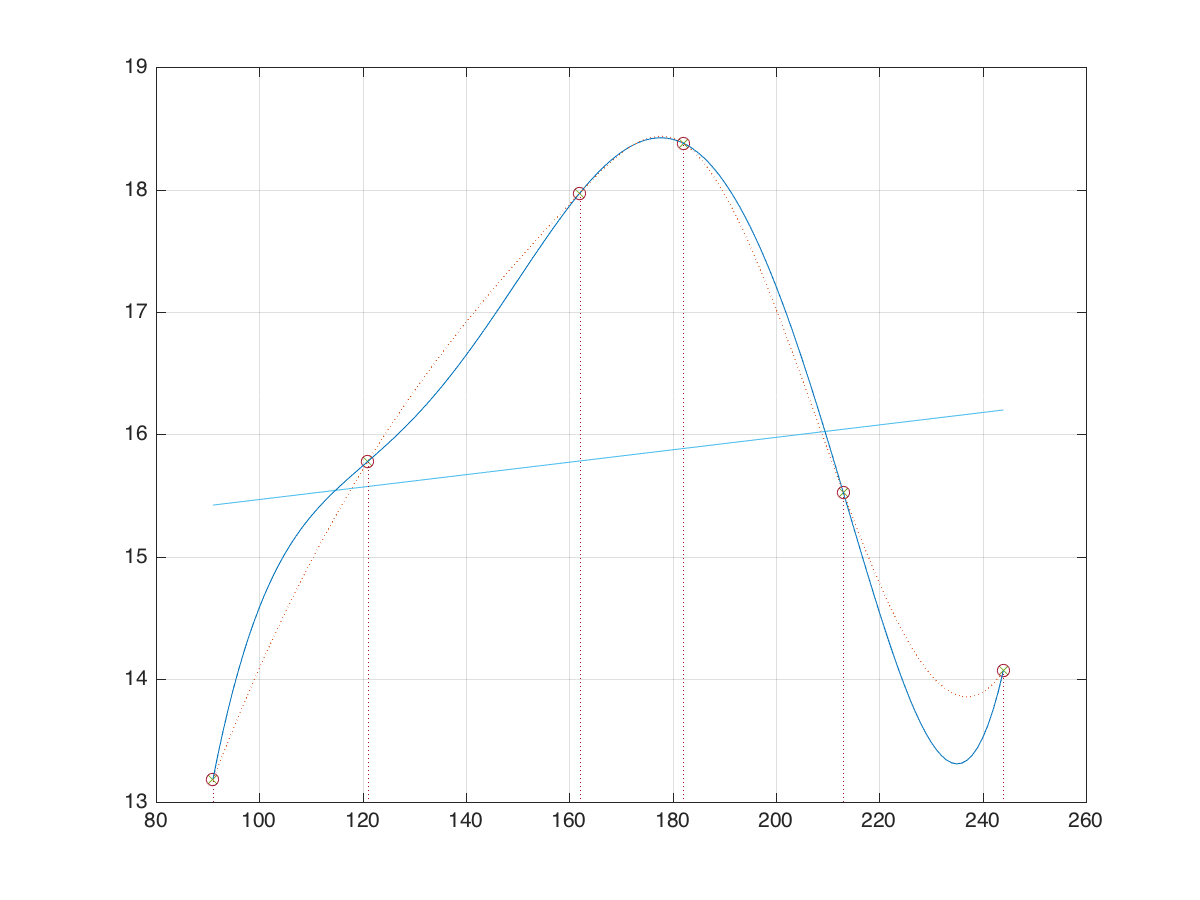
\includegraphics{fig1a.png}
\caption{Anpassning med femtegradspolynom och med spline (streckad
linje)\label{fig:fig1a}}
\end{figure}

\begin{Shaded}
\begin{Highlighting}[]
\NormalTok{x = [}\FloatTok{91} \FloatTok{121} \FloatTok{162} \FloatTok{182} \FloatTok{213} \FloatTok{244}\NormalTok{]';}
\NormalTok{y = [}\FloatTok{13.18} \FloatTok{15.78} \FloatTok{17.97} \FloatTok{18.38} \FloatTok{15.53} \FloatTok{14.07}\NormalTok{]';}
\NormalTok{A = [ones(}\FloatTok{6}\NormalTok{,}\FloatTok{1}\NormalTok{) x x.^}\FloatTok{2} \NormalTok{x.^}\FloatTok{3} \NormalTok{x.^}\FloatTok{4} \NormalTok{x.^}\FloatTok{5}\NormalTok{];}
\NormalTok{c = A \textbackslash{} y;}
\NormalTok{X = x(}\FloatTok{1}\NormalTok{):x(}\FloatTok{6}\NormalTok{);}
\NormalTok{P = c(}\FloatTok{1}\NormalTok{) + c(}\FloatTok{2}\NormalTok{)*X + c(}\FloatTok{3}\NormalTok{)*X.^}\FloatTok{2} \NormalTok{+ c(}\FloatTok{4}\NormalTok{)*X.^}\FloatTok{3} \NormalTok{+ c(}\FloatTok{5}\NormalTok{)*X.^}\FloatTok{4} \NormalTok{+ c(}\FloatTok{6}\NormalTok{)*X.^}\FloatTok{5}\NormalTok{;}
\NormalTok{stem(x, y, }\StringTok{':'}\NormalTok{)}
\NormalTok{hold on}
\NormalTok{axis([}\FloatTok{80}\NormalTok{, }\FloatTok{260}\NormalTok{, }\FloatTok{13}\NormalTok{, }\FloatTok{19}\NormalTok{])}
\NormalTok{plot(X, P), grid}
\NormalTok{Pm = spline(x, y, X);}
\NormalTok{hold on}
\NormalTok{plot(X, Pm, }\StringTok{':'}\NormalTok{)}
\NormalTok{P(}\FloatTok{157} \NormalTok{- }\FloatTok{90}\NormalTok{)}
\NormalTok{P(}\FloatTok{227} \NormalTok{- }\FloatTok{90}\NormalTok{)}
\end{Highlighting}
\end{Shaded}

Solens uppetid en viss dag finns i \texttt{P(dagnr\ -\ 90)}. Det ger att
6 juni (dag~157) var solen uppe 17.69~h, och 15 augusti (dag~227) var
den uppe 13.73~h.

\subsection{Uppgift 1b}\label{uppgift-1b}

Här har jag använt \textsc{matlab}s \texttt{polyfit} och
\texttt{polyval} för att anpassa ett andragradspolynom till
mätpunkterna. Soltiden för den 6~juni blir 17.73~h med denna modell. Se
figur \ref{fig:fig1b}.

\begin{figure}[htbp]
\centering
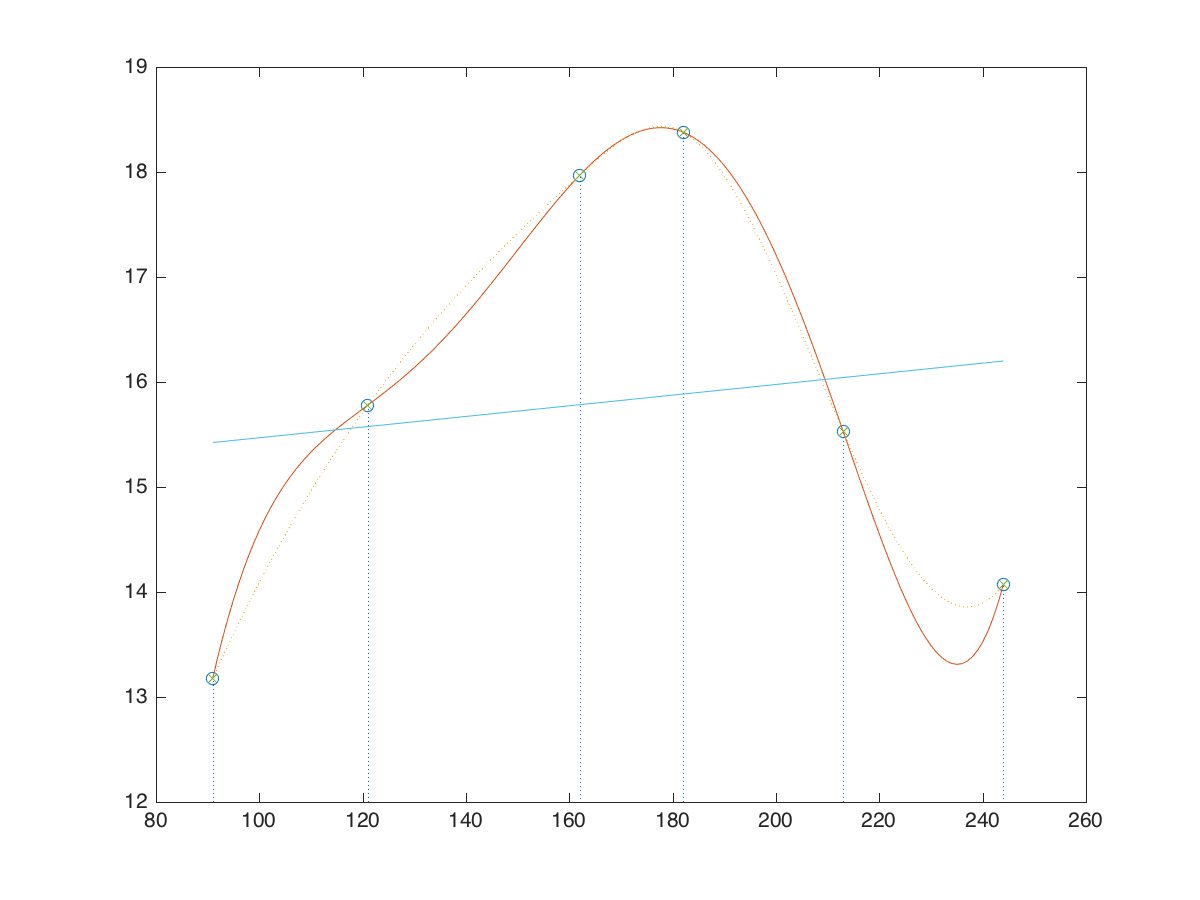
\includegraphics{fig1b.png}
\caption{Anpassning med andragradspolynom\label{fig:fig1b}}
\end{figure}

\begin{Shaded}
\begin{Highlighting}[]
\NormalTok{x = [}\FloatTok{91} \FloatTok{121} \FloatTok{162} \FloatTok{182} \FloatTok{213} \FloatTok{244}\NormalTok{]';}
\NormalTok{y = [}\FloatTok{13.18} \FloatTok{15.78} \FloatTok{17.97} \FloatTok{18.38} \FloatTok{15.53} \FloatTok{14.07}\NormalTok{]';}
\NormalTok{d = polyfit(x, y, }\FloatTok{2}\NormalTok{);}
\NormalTok{X = x(}\FloatTok{1}\NormalTok{):x(}\FloatTok{6}\NormalTok{);}
\NormalTok{P = polyval(d, xplot);}
\NormalTok{plot(x, y, }\StringTok{'x'}\NormalTok{, X, P), grid}
\end{Highlighting}
\end{Shaded}

\subsection{Uppgift 1c}\label{uppgift-1c}

Här använder vi som modellfunktion
\(c_1 + c_2 \cos{\omega t} + c_3 \sin{\omega t},\quad \omega = 2\pi/365\)
Eftersom vi har cykliska data med en period på 365 dagar bör det ge en
god anpassning. Data har kompletterats så hela året är täckt.
Residualkurvan har plottats separat. Resultatet visas i figur
\ref{fig:fig1c}.

Felkvadratsumman fås som \(\mathbf{r}^T \mathbf{r}\), där \(\mathbf{r}\)
är residualvektorn, och är \(1.9750\). Nationaldagens soltid är
\texttt{F(157)} \(= 17.7654\).

\begin{figure}[htbp]
\centering
\includegraphics{fig1c.png}
\caption{Anpassning med trigonometriskt uttryck\label{fig:fig1c}}
\end{figure}

\begin{Shaded}
\begin{Highlighting}[]
\CommentTok{% lade till dag 365 med samma värde som dag 1}
\NormalTok{x = [}\FloatTok{1} \FloatTok{32} \FloatTok{60} \FloatTok{91} \FloatTok{121} \FloatTok{162} \FloatTok{182} \FloatTok{213} \FloatTok{244} \FloatTok{274} \FloatTok{305} \FloatTok{335} \FloatTok{365}\NormalTok{]';}
\NormalTok{y = [}\FloatTok{6.13} \FloatTok{8.02} \FloatTok{10.42} \FloatTok{13.18} \FloatTok{15.78} \FloatTok{17.97} \FloatTok{18.38} \FloatTok{15.53} \FloatTok{14.07} \FloatTok{11.43} \FloatTok{8.73} \FloatTok{6.55} \FloatTok{6.13}\NormalTok{]';}
\NormalTok{w = }\FloatTok{2} \NormalTok{* pi / }\FloatTok{365}\NormalTok{;}
\NormalTok{A = [ones(}\FloatTok{13}\NormalTok{, }\FloatTok{1}\NormalTok{) cos(w*x) sin(w*x)];}
\NormalTok{c = A \textbackslash{} y;}
\NormalTok{X = x(}\FloatTok{1}\NormalTok{):x(}\FloatTok{13}\NormalTok{);}
\NormalTok{F = c(}\FloatTok{1}\NormalTok{) + c(}\FloatTok{2}\NormalTok{) * cos(w*X) + c(}\FloatTok{3}\NormalTok{) * sin(w*X);}
\NormalTok{r = y - A * c;   }\CommentTok{% residual}
\NormalTok{fkvsum = r' * r  }\CommentTok{% felkvadratsumma}
\NormalTok{F(}\FloatTok{157}\NormalTok{)           }\CommentTok{% 6 juni}
\NormalTok{subplot(}\FloatTok{1}\NormalTok{, }\FloatTok{2}\NormalTok{, }\FloatTok{1}\NormalTok{)}
\NormalTok{plot(x, y, }\StringTok{'r:o'}\NormalTok{, X, F), grid}
\NormalTok{title(}\StringTok{'Anpassning med trigonometriskt uttryck'}\NormalTok{)}
\NormalTok{subplot(}\FloatTok{1}\NormalTok{, }\FloatTok{2}\NormalTok{, }\FloatTok{2}\NormalTok{)}
\NormalTok{plot(x, r), grid}
\NormalTok{title(}\StringTok{'Residualkurva'}\NormalTok{)}
\end{Highlighting}
\end{Shaded}

\section{2. Numerisk derivering och
noggrannhetsordning}\label{numerisk-derivering-och-noggrannhetsordning}

\end{document}
